% $Id: template.tex 11 2007-04-03 22:25:53Z jpeltier $

\documentclass{vgtc}                          % final (conference style)
%\documentclass[review]{vgtc}                 % review
%\documentclass[widereview]{vgtc}             % wide-spaced review
%\documentclass[preprint]{vgtc}               % preprint
%\documentclass[electronic]{vgtc}             % electronic version

%% Uncomment one of the lines above depending on where your paper is
%% in the conference process. ``review'' and ``widereview'' are for review
%% submission, ``preprint'' is for pre-publication, and the final version
%% doesn't use a specific qualifier. Further, ``electronic'' includes
%% hyperreferences for more convenient online viewing.

%% Please use one of the ``review'' options in combination with the
%% assigned online id (see below) ONLY if your paper uses a double blind
%% review process. Some conferences, like IEEE Vis and InfoVis, have NOT
%% in the past.

%% Figures should be in CMYK or Grey scale format, otherwise, colour 
%% shifting may occur during the printing process.

%% These few lines make a distinction between latex and pdflatex calls and they
%% bring in essential packages for graphics and font handling.
%% Note that due to the \DeclareGraphicsExtensions{} call it is no longer necessary
%% to provide the the path and extension of a graphics file:
%% \includegraphics{diamondrule} is completely sufficient.
%%
\ifpdf%                                % if we use pdflatex
  \pdfoutput=1\relax                   % create PDFs from pdfLaTeX
  \pdfcompresslevel=9                  % PDF Compression
  \pdfoptionpdfminorversion=7          % create PDF 1.7
  \ExecuteOptions{pdftex}
  \usepackage{graphicx}                % allow us to embed graphics files
  \DeclareGraphicsExtensions{.pdf,.png,.jpg,.jpeg} % for pdflatex we expect .pdf, .png, or .jpg files
\else%                                 % else we use pure latex
  \ExecuteOptions{dvips}
  \usepackage{graphicx}                % allow us to embed graphics files
  \DeclareGraphicsExtensions{.eps}     % for pure latex we expect eps files
\fi%

%% it is recomended to use ``\autoref{sec:bla}'' instead of ``Fig.~\ref{sec:bla}''
\graphicspath{{figures/}{pictures/}{images/}{./}} % where to search for the images

\usepackage{amsmath}
\usepackage{microtype}                 % use micro-typography (slightly more compact, better to read)
\PassOptionsToPackage{warn}{textcomp}  % to address font issues with \textrightarrow
\usepackage{textcomp}                  % use better special symbols
\usepackage{mathptmx}                  % use matching math font
\usepackage{times}                     % we use Times as the main font
\renewcommand*\ttdefault{txtt}         % a nicer typewriter font
\usepackage{cite}                      % needed to automatically sort the references
\usepackage{tabu}                      % only used for the table example
\usepackage{booktabs}                  % only used for the table example
%% We encourage the use of mathptmx for consistent usage of times font
%% throughout the proceedings. However, if you encounter conflicts
%% with other math-related packages, you may want to disable it.

% % Packages inserted by Brian
% \usepackage{caption}
% \usepackage{subcaption}


%% If you are submitting a paper to a conference for review with a double
%% blind reviewing process, please replace the value ``0'' below with your
%% OnlineID. Otherwise, you may safely leave it at ``0''.
\onlineid{0}

%% declare the category of your paper, only shown in review mode
\vgtccategory{Research}

%% allow for this line if you want the electronic option to work properly
\vgtcinsertpkg

%% In preprint mode you may define your own headline.
%\preprinttext{To appear in an IEEE VGTC sponsored conference.}

%% Paper title.

\title{Tsunami Inundation Visualization}

%% This is how authors are specified in the conference style

%% Author and Affiliation (single author).
%%\author{Roy G. Biv\thanks{e-mail: roy.g.biv@aol.com}}
%%\affiliation{\scriptsize Allied Widgets Research}

%% Author and Affiliation (multiple authors with single affiliations).
%%\author{Roy G. Biv\thanks{e-mail: roy.g.biv@aol.com} %
%%\and Ed Grimley\thanks{e-mail:ed.grimley@aol.com} %
%%\and Martha Stewart\thanks{e-mail:martha.stewart@marthastewart.com}}
%%\affiliation{\scriptsize Martha Stewart Enterprises \\ Microsoft Research}

%% Author and Affiliation (multiple authors with multiple affiliations)
\author{Kellie MacPhee\thanks{e-mail: kmacphee@uw.edu}\\ %
    \scriptsize Mathematics %
\and Brian de Silva\thanks{e-mail: bdesilva@uw.edu}\\ %
    \scriptsize Applied Mathematics %
\and Abraham Engle\thanks{e-mail: aengle2@uw.edu}\\ %
    \scriptsize Mathematics %
\and Benjamin Liu\thanks{e-mail: benliu@uw.edu}\\ %
    \scriptsize Applied Mathematics
}

%% A teaser figure can be included as follows, but is not recommended since
%% the space is now taken up by a full width abstract.
%\teaser{
%  \includegraphics[width=1.5in]{sample.eps}
%  \caption{Lookit! Lookit!}
%}

%% Abstract section.
\abstract{Numerical simulations are used to model and predict the impact of tsunamis. By simulating many possible tsunamis and estimating their probability of occurrence, the probability of exceeding a given level of inundation (flooding) can be estimated for every point in the landscape, giving rise to a hazard map. Visualizing hazard maps is difficult for several reasons. First, the data has a large amount of uncertainty: the probability of each simulated event must be estimated; and the hazard maps are generated from a limited pool of simulated events, and so may not be representative of the worst or most exotic tsunamis. Second, the resultant hazard maps do not specify a unique inundation level at every point, but rather a hazard function that gives the probability of inundation at all possible depths.
\\ \\
To effectively communicate the dangers and potential impacts of tsunamis to the general public, we employ interactive and research-based design techniques to facilitate users' understanding of the complex data. We display contour plots of inundation level for a fixed probability and allow the users to manipulate the probability to see how inundation changes over the landscape. We also use small multiples to present the user with an overview of the inundation from a sample of individual simulations, showing a sampling of possible outcomes from separate events. Our hope is that by showing both the aggregate data and the data from individual simulations, we can reduce the abstraction in the uncertainty measures that are typically reported. To further improve user comprehension of our data, provide context, and generate interest we embed our visualizations in an article-style narrative structure.} % end of abstract

% On a 250 x 250 (lon,lat) grid with lower left corner  (235.79781, 41.739671) and upper-right corner (235.82087, 41.762726)

%% ACM Computing Classification System (CCS). 
%% See <http://www.acm.org/about/class> for details.
%% We recommend the 2012 system <http://www.acm.org/about/class/class/2012>
%% For the 2012 system use the ``\CCScatTwelve'' which command takes four arguments.
%% The 1998 system <http://www.acm.org/about/class/class/2012> is still possible
%% For the 1998 system use the ``\CCScat'' which command takes four arguments.
%% In both cases the last two arguments (1998) or last three (2012) can be empty.

% \CCScatlist{
%   \CCScatTwelve{Human-centered computing}{Visu\-al\-iza\-tion}{Visu\-al\-iza\-tion techniques}{Treemaps};
% }

%\CCScatlist{
  %\CCScat{H.5.2}{User Interfaces}{User Interfaces}{Graphical user interfaces (GUI)}{};
  %\CCScat{H.5.m}{Information Interfaces and Presentation}{Miscellaneous}{}{}
%}

%% Copyright space is enabled by default as required by guidelines.
%% It is disabled by the 'review' option or via the following command:
% \nocopyrightspace

%%%%%%%%%%%%%%%%%%%%%%%%%%%%%%%%%%%%%%%%%%%%%%%%%%%%%%%%%%%%%%%%
%%%%%%%%%%%%%%%%%%%%%% START OF THE PAPER %%%%%%%%%%%%%%%%%%%%%%
%%%%%%%%%%%%%%%%%%%%%%%%%%%%%%%%%%%%%%%%%%%%%%%%%%%%%%%%%%%%%%%%%

\begin{document}

%% The ``\maketitle'' command must be the first command after the
%% ``\begin{document}'' command. It prepares and prints the title block.

%% the only exception to this rule is the \firstsection command
\firstsection{Introduction}
\maketitle
% ``An explanation of the problem and the motivation for solving it.''

% {\bf Outline:}
% \begin{enumerate}
%     \item A bit of background on probabilistic tsunami hazard modeling
%     \item Explicit description of the problems our work seeks to address
%     \begin{enumerate}
%         \item Hazard maps and the data used to produce them contain multiple sources of uncertainty. It is difficult to communicate this uncertainty in an intuitive way.
%         \item Hazard maps are inherently complex and nuanced and can therefore be difficult for non-experts to decipher.
%     \end{enumerate}
%     \item Motivation for solving these problems?
% \end{enumerate}

Coastal cities along the West Coast are particularly susceptible to damage caused by tsunamis.
In this project we focus on \emph{Crescent City}, a coastal town in California with a history of extreme damage from tsunamis. To improve Crescent City’s preparedness researchers seek to better understand the impact of tsunamis arising from a number of possible seismic events. One approach is to use numerical simulations to predict tsunami damage. The process of modeling a tsunami begins with the specification of a seismic event that causes a tsunami. This entails stipulating the location of the earthquake and a slip pattern that measures where and to what degree the ocean floor moves during the earthquake. The slip pattern determines how water is displaced, leading to the initial formation of the tsunami. Numerical simulation is used to track the displaced water and the resultant waves from the epicenter of the seismic event, across the ocean, and to the Crescent City harbor to determine the degree of inland flooding, known as inundation.

Researchers at the University of Washington conducted a suite of simulations as part of a workshop to further develop the technology underlying probabilistic hazard maps. We worked with data from a set of 13 numerical simulations. Each simulation corresponds to a single seismic event. For each event, the simulations were used to obtain the maximum inundation levels in a $250\times250$ grid centered over Crescent City harbor (at approximately (41.7558,-124.2026) in decimal degrees (DD)). Associated with each seismic event is its \emph{annual probability of occurrence}, which are in practice estimated by experts. For simplicity, researchers typically assume that earthquakes are independent; however, there is likely some correlation between seismic events (e.g. one would not expect two large earthquakes to occur in a row, but smaller aftershocks are quite common).

Detailed numerical simulations are computationally expensive and time-consuming to produce.
It is not uncommon for scientists to have access to only a small number of simulated events. Seismic events as far away as Asia can induce tsunamis that strike the West Coast. To simulate damage from such events, one must propagate the resulting tsunamis across the entire ocean and into Crescent City harbor. %Doing so accurately makes these simulations extremely computationally costly.

\subsection{Types of visualizations}

There are three types of visualizations that are typically used to convey the results of tsunami simulations. For this project we focus on the following.

Given the annual probability of each simulated tsunami and fixing a point on the grid we can compute the annual probability of inundation exceeding any particular level. Allowing the inundation level to vary, we can construct what is known as a \emph{hazard curve}: a one-dimensional curve showing the predicted annual probability of the water reaching different levels at a fixed point in space. Figure \ref{fig:hazard-curve} shows a set of three hazard curves, each corresponding to a different subset of the numerical simulations. The annual probability is plotted on the y-axis and the inundation level (or exceedance level) is plotted on the x-axis.

\begin{figure}[b!]
    \centering
    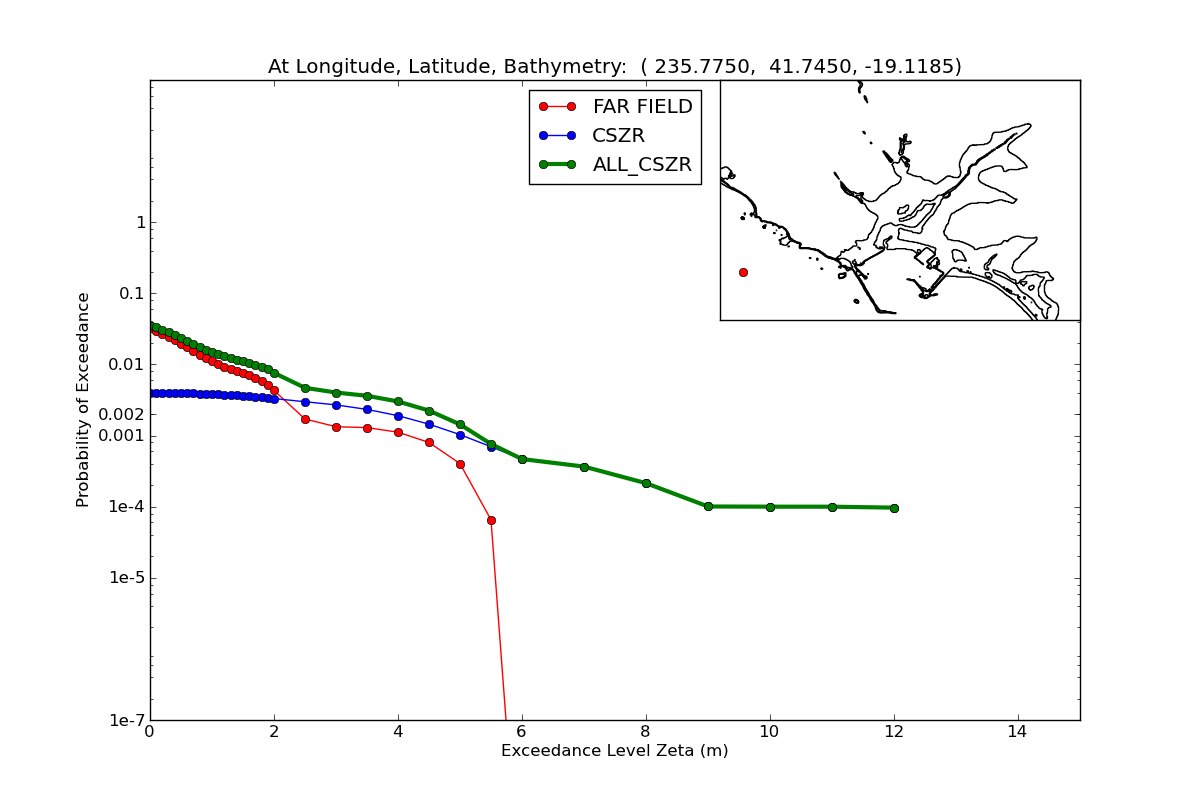
\includegraphics[width=\columnwidth]{pictures/HazardCurveFarCascacadiaAll_GridPoint_093474.png}
    \caption{Three hazard curves, each corresponding to a different subset of the numerical simulations. The spatial point whose hazard curves are plotted is shown as a red dot in the map in the upper-right.}
    \label{fig:hazard-curve}
\end{figure}

Fixing an annual probability, allowing the spatial point to vary, and plotting the associated inundation levels from the hazard curves, we obtain a \emph{hazard map}. Figure \ref{fig:hazard-map} shows an example hazard map generated by the research team who we collaborated with on this project. One of the team's goals is to effectively communicate their findings to the general public. However, accurately interpreting hazard maps and their siblings can be challenging for people without technical backgrounds.

\begin{figure}[t!]
    \centering
    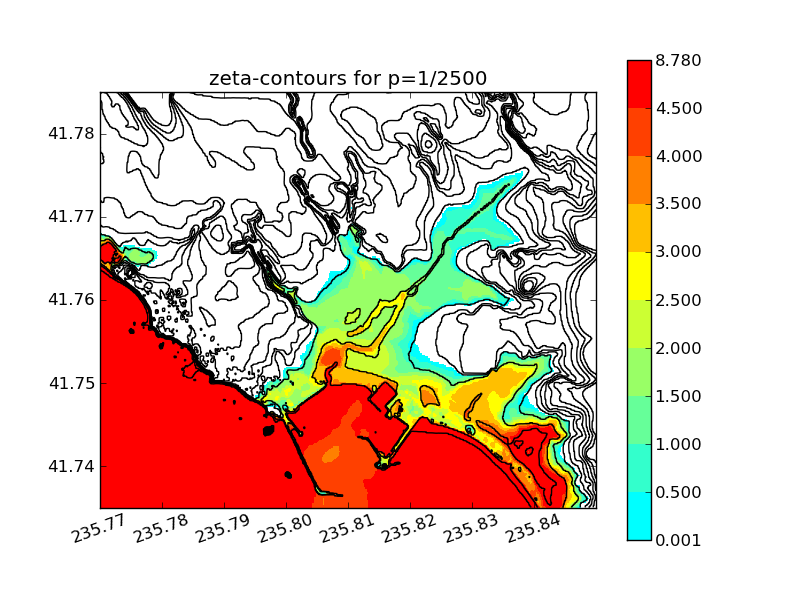
\includegraphics[width=\columnwidth]{pictures/zeta-contours_prob_0004.png}
    \caption{A hazard map for the Crescent City harbor area with annual probability set to $p=1/2500$. The inundation level has been encoded via color.}
    \label{fig:hazard-map}
\end{figure}

Furthermore, there are multiple {\it sources of uncertainty} (both aleatoric and epistemic) that feed into hazard maps:
\begin{enumerate}
    \item Estimation of annual probability of different seismic events;
    \item Variability of outcomes over a small number of events;
    \item Error due to the assumption that the seismic events are independent;
    \item Error in the numerical simulations of tsunamis.
\end{enumerate}
Researchers would especially like to be able to communicate the uncertainty inherent in tsunami simulations to a general audience.

Our goals for this project are twofold. First, we would like to present hazard maps in a manner that is easily intelligible for non-experts. Second, we seek to convey the uncertainty underlying hazard maps in an intuitive way.

% \begin{equation}
%     \zeta = \begin{cases}
%     h & \text{if } B > 0,\\
% \eta:=h + B & \text{if } B \le 0.
% \end{cases}
% \end{equation}

% $\eta$ is sea-surface elevation relative to MHW, $\zeta$ is maximum observed value of tsunami
%% \section{Introduction} %for journal use above \firstsection{..} instead

The remainder of this report is organized as follows. We give an overview of related work from the data visualization community in Section \ref{sec:related-work}. In Section \ref{sec:methods} we discuss the methods employed to address the problems stated above. We present some preliminary results in Section \ref{sec:results} and discuss insights drawn from them in Section \ref{sec:discussion}. Finally, we describe how our work could be extended and/or improved in Section \ref{sec:future-work}.

\section{Related Work}\label{sec:related-work}
% ``A description of prior research or work related to your project.''

The outcomes of the simulations were previously communicated in the technical report \cite{gonzalez2013probabilistic}. Typical visualizations in this work are similar to Figure~\ref{fig:hazard-map}, and the report is aimed at a technical audience. One of our main goals is to extend these visualizations to be accessible to a general audience with little to no statistical background.

Much work has been done on improving visualizations involving uncertainty, but there is still little consensus within the field on best practices, and the appropriate techniques often depend on the context (e.g. audience type, uncertainty type).
Hypothetical outcome plots (HOPs) were introduced in \cite{hypothetical} as a way to help viewers understand the uncertainty inherent in data presented. The authors advocate for representing probability distributions using animations that cycle through a sample of discrete possible outcomes as an alternative to static visualizations such as error bars or violin plots. HOPs were shown to outperform error bars and violin plots for judgments about plots of two and three quantities. HOPs were designed in particular for communicating information about probabilities to audiences with limited statistical backgrounds.
Follow-up work in \cite{hullman2018imagining} established that "visualizing uncertainty as a set of discrete outcomes, as opposed to a continuous
probability distribution, could improve recall of a sampling distribution from a single experiment."
We draw on HOPs as inspiration for the flipbook part of our visualization (details in Section \ref{sec:flipbook}).



% Example figure:

% \begin{figure}[tb]
%  \centering % avoid the use of \begin{center}...\end{center} and use \centering instead (more compact)
%  \includegraphics[width=\columnwidth]{paper-count-w-2015-new}
%  \caption{A visualization of the 1990--2015 data from \autoref{tab:vis_papers}. The image is from \cite{Isenberg:2017:VMC} and is in the public domain.}
%  \label{fig:sample}
% \end{figure}


\section{Methods}\label{sec:methods}
Our visualizations are implemented in HTML and JavaScript using the D3 framework. The maps in our visualization are built using the Google Maps API. Throughout, inundation levels are overlaid on the maps as shaded contour plots, with color encoding water depth above normal (meters). We select a color palette with colors that are distinguishable for every type of color-blindness. Dark blue and purple intuitively correspond to deeper water and yellowish greens to milder levels of flooding. We employ a number of narrative and design techniques to achieve our goals.

\subsection{Narrative}
We embed our visualizations within a larger narrative structure to make them more digestible. In particular, we adopt the ``magazine style'' approach of Segel and Heer \cite{segel2010narrative}. We begin with an anecdote that emphasizes the usefulness of numerical simulations to grab the reader's attention. Preceding each visualization is a short body of text explaining both the rationale behind showing the visualization and providing information to prime the reader so that they can more effectively interpret the visualization. Following each we provide some useful observations to help ensure readers do not miss out on any insights we think they should make. The narrative format of our web page, paired with the interactivity of our visualizations, guides readers' thinking through the complexities of probabilistic hazard mapping while allowing them the flexibility to explore the data and draw their own conclusions.

\subsection{Flipbook}\label{sec:flipbook}
The first visualization piece we present to viewers is a flipbook-style animation that rotates through the full set of 13 simulations, showing the effects of each on the map. The flipbook was inspired by the sampling-based visualizations of uncertainty at the Interactive Data Lab at the University of Washington \cite{hullman2018imagining}. Seeing the results of all the simulations gives the viewer an implicit introduction to the variability present in the data. We have a relatively small number of simulations (13), many with very different outcomes, and the likelihood of each event can vary by orders of magnitude. In order to show a range of possible events including the most extreme simulations (rather than, say, showing simulations at rates proportional to their annual probabilities), we postpone considerations of the likelihood of each event for the aggregate maps and probability explorer to follow. We include a silhouette of a person of average height beside the legend to give readers unaccustomed to reasoning in meters (the unit used in the simulations) a better idea of the scale of the flooding depth.

\subsection{Aggregate inundation map}\label{sec:aggregate-map}
While it can be enlightening to examine the results of individual simulations, readers who wish the act on this information need a way to consolidate outcomes from many simulations. This is accomplished by combining the results of individual simulations into an aggregate hazard map. The aggregate map shows expected inundation level over all simulated events for a fixed probability. Users can interact with this map by panning, zooming, and pinpointing areas of interest. A slider allows users to vary the probability threshold used to create the map.
Users can also choose to filter the simulations that are shown based on the type of seismic event modeled: near-field (Cascadia subduction zone), far-field (other origin) events, or both. These sets of events vary in severity and likelihood.

\subsection{Small multiples}\label{sec:small-multiples}
Our main visualization introduces the aggregate inundation map but also connects the aggregate data to individual simulations through small multiple representations of six simulations. The small multiples convey a broad range of possible outcomes in the event of a tsunami. Showing specific events highlights the variety of possible outcomes, ensuring that extreme events are not lost in the aggregate map. The small multiples also allow the reader to make direct comparisons between simulations, which is difficult to accomplish using the flipbook. Labels describe the plotted seismic events and give annual probabilities for each, providing additional context. The small multiples are shown opposite the aggregate inundation map to facilitate further comparison and encouraging users to observe how different simulation results factor into the aggregate map. Selecting an area in the aggregate map causes the small multiples to pan and center to the same location so that simulation results in areas of interest can quickly be examined and compared.



\subsection{Interactive probability explorer}\label{sec:prob-explorer}
Often users are concerned with the likelihood of a tsunami over a number of years, not the probability one will occur in the next year. For example, one might wonder: over the 30 years I expect to live in this house, what are the chances I will experience significant flooding due to a tsunami?

Going from the annual probability of an event (or collection of events) to the probability over a number of years is slightly nuanced. To mitigate user confusion about annual probabilities and to help users reason effectively about long-term risks, we provide an interactive probability explorer. This explorer allows readers to enter an annual probability, $p$, and a number of years, $N$. It then returns the probability that at least one event (or collection of events) with annual probability $p$ will occur over a period of $N$ years. The interactive nature of the calculator allows users to enter annual probabilities from simulations that stood out to them from the small multiples graphic or from the hazard map and more accurately compute the likelihood of such events over time.

\section{Results}\label{sec:results}
% ``The visualizations your system produces and any data to help evaluate your approach. For example, you might describe a case study that illustrates how your visualization(s) address your chosen problem.''

In this section, we present the visualizations produced for our project. Dynamic versions can be found on our project website. All visualizations are embedded in an article-like web page. A static version of the flipbook visualization described in Section \ref{sec:flipbook} is shown in Figure \ref{fig:flipbook}. Each simulation image is shown for about two seconds before fading out and a new run fading in. The combined hazard map and small multiples visualization is given in Figure \ref{fig:whole-vis}. In this image the user has clicked on the point enclosed by the red circles in the seven plots, causing the small multiples maps to shift their centers from the default position to this point. Figure \ref{fig:prob-explorer} illustrates how our probability explorer from Section \ref{sec:prob-explorer} functions.


\begin{figure}
    \centering
    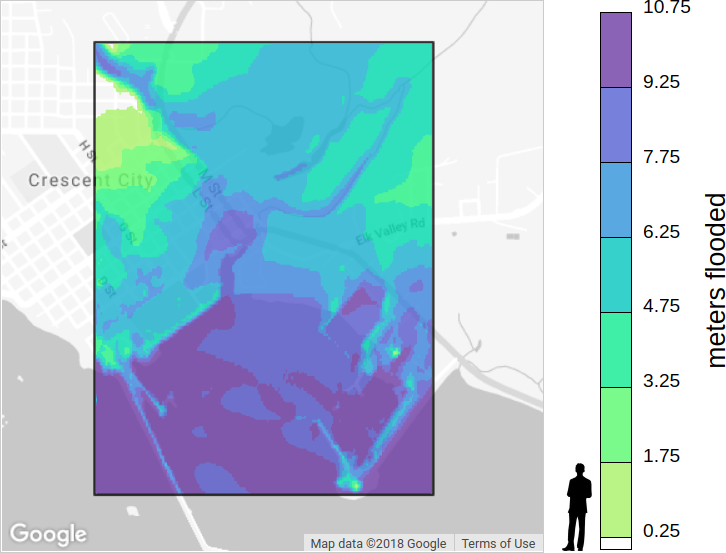
\includegraphics[width=\columnwidth]{pictures/flipbook.png}
    \caption{A static image of our flipbook animation.}
    \label{fig:flipbook}
\end{figure}


\begin{figure}
    \centering
    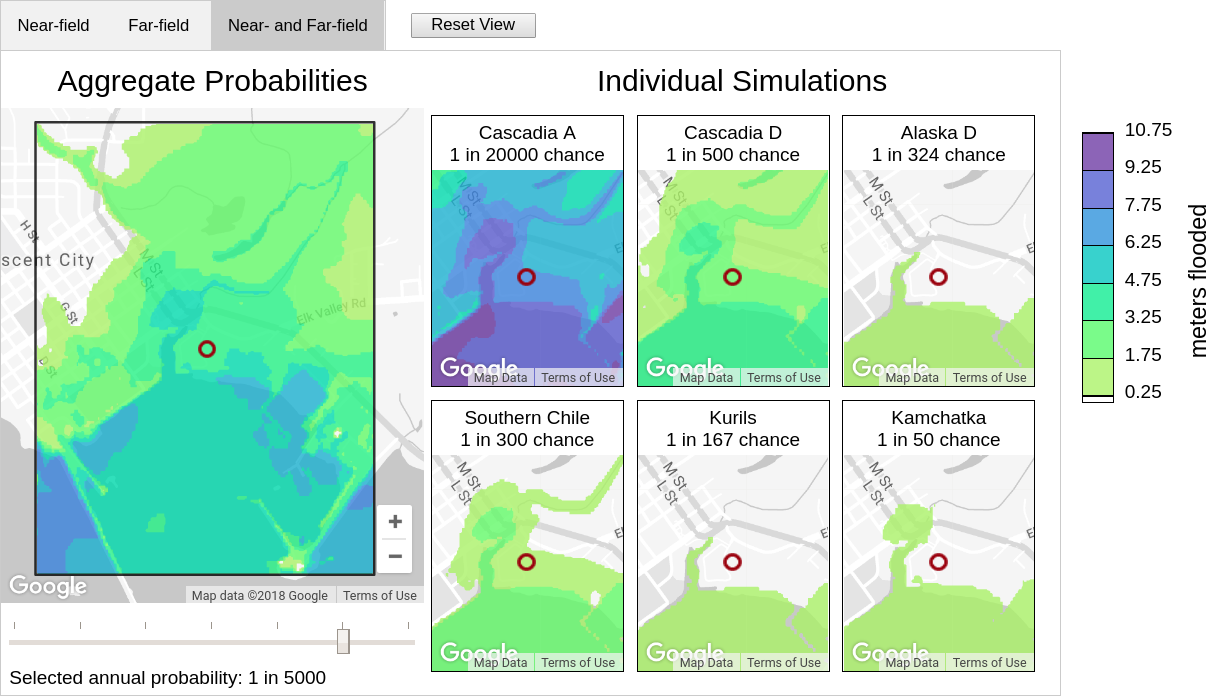
\includegraphics[width=\columnwidth]{pictures/wholevis.png}
    \caption{An aggregate inundation map beside small multiples of some of the simulations used to construct it}
    \label{fig:whole-vis}
\end{figure}


\begin{figure}
    \centering
    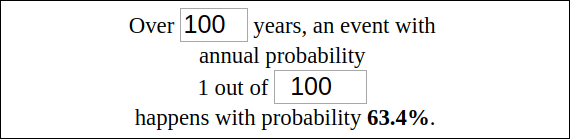
\includegraphics[width=\columnwidth]{pictures/prob_explorer.png}
    \caption{Our probability explorer}
    \label{fig:prob-explorer}
\end{figure}

Throughout the process, our visualization continually evolved based on both computational considerations and design considerations. For example, we originally performed contour mapping in Python and then imported the results to draw using D3. After difficulties with getting the contours correct, however, we switched to more heavily relying on the Google Maps API for processing the data. Design considerations such as the color scheme, the marker choice for the user-clicked focus point in the aggregate map (currently a red circle), and the decision to include the flipbook and probability explorer as separate components of the visualization, also evolved over time. Many of these decisions were based on user feedback, including feedback during the project milestone review, and we believe they have significantly improved the overall result.

\section{Discussion}\label{sec:discussion}
% ``What has the audience learned from your work? What new insights or practices has your system enabled? A full blown user study is not expected, but informal observations of use that help evaluate your system are encouraged.''

Users who have read through our interactive article reported an increased understanding of tsunami simulations and the uncertainties behind them, better interpretation of tsunami hazard maps, and a better understanding of the annual probabilities and how these quantities factor into emergency preparedness.

Users unfamiliar with the topic had several insights after viewing our final product:
\begin{itemize}
    \item There is a lot of uncertainty surrounding whether actual earthquakes will resemble those that were simulated. 
    \item The simulated events have very low estimated probabilities of occurring. %(Andreas)
    \item Understanding the meaning of annual probabilities is challenging, and the probability explorer is helpful with grappling with this concept and making it more understandable.
\end{itemize}

Suggestions provided by users for improving the existing interface included:
\begin{itemize}
    \item Adding the ability to zoom within the small multiples.
    \item Adding captions to the flipbook, specifying details of the simulation currently being shown.
\end{itemize}

%Although we did not have time to address these concerns before the final project deadline, they are reasonably small changes and we hope to address them in the future with our collaborators.

\section{Future Work}\label{sec:future-work}

Dan Abramson, Associate Professor of Urban Design and Planning at the University of Washington, plans to test the impact of our visualizations in a participatory GIS exercise with members of the public. Our visualization will be compared to other existing visualizations of the same data, in regards to user perceptions of uncertainty and tsunami risk. We look forward to this extension of our work, and the chance to see its effectiveness on a broader scale.

There are a number of additional ways that the current work could be extended, as well:
\begin{itemize}
    \item With additional simulations, the map could cover a greater geographic region, including additional cities.
    \item Including additional simulations would reduce uncertainty and give a better sense of possible outcomes.
    \item By using alternative encodings of uncertainty, results may be made more readily interpretable. In addition, it would be interesting to evaluate the usefulness of the interactive probability explorer in a controlled study with human subjects, particularly as to whether inundation, probabilistic, or both are more digestible for the average coastal resident. %TODO maybe delete
\end{itemize}
\acknowledgments
{
    The authors would like to thank Professor \href{http://faculty.washington.edu/rjl}{Randy LeVeque} for suggesting the project and for the providing the data that went into the tsunami simulations.
	The \href{https://digital.lib.washington.edu/researchworks/handle/1773/25916}{technical report} and \href{https://github.com/rjleveque/ptha_tutorial}{Github repository} were invaluable tools in our effort to complete this project.
	We would also like to thank Professors \href{https://evans.uw.edu/profile/bostrom}{Ann Bostrom} and \href{http://urbdp.be.washington.edu/people/dan-abramson/}{Dan Abramson} for their helpful discussions and Professor Heer and Halden for their feedback during the milestone review.
			
    On the coding side, Mike Bostock's \href{https://github.com/d3/d3-scale-chromatic}{d3-scale-chromatic} \cite{d3-scale-chromatic} 
    and Susie Lu's \href{http://d3-legend.susielu.com/}{d3-legend} \cite{d3-legend} were extremely helpful in producing a polished finished product.
    We also made heavy use of examples from the \href{https://www.w3schools.com/}{w3schools}.
    Of course, none of this would have been possible without the Google Maps API and D3.
    And finally, we would like to thank the A3-wildfires group (Charlie Godfrey, Kelsey Maass, Connor Sawaske, and Saumya Sinha) for their instrumental help in getting us started on using the Google Maps API with D3.
}
%\bibliographystyle{abbrv}
\bibliographystyle{abbrv-doi}
%\bibliographystyle{abbrv-doi-narrow}
%\bibliographystyle{abbrv-doi-hyperref}
%\bibliographystyle{abbrv-doi-hyperref-narrow}

\bibliography{bibliography}
\end{document}
